\begin{abstract}
The peracarid taxon Cumacea is an essential indicator of benthic quality in marine ecosystems. This study investigated the influence of environmental (i.e., biological or ecosystemic), climatic (i.e., meteorological or atmospheric), and geographic (i.e., spatial or regional) attributes on their genetic variability in the Northern North Atlantic, focusing on Icelandic waters. We analyzed partial sequences of the 16S rRNA mitochondrial gene from 62 Cumacea specimens. Using the \textit{aPhyloGeo} software, we compared these sequences with relevant parameters such as latitude (decimal degree) at the end of sampling, wind speed (m/s) at the start of sampling, O\textsubscript{2} concentration (mg/L), and depth (m) at the start of sampling.

Our analyses revealed variability in most spatial and biological attributes, reflecting the diversity of ecological requirements and benthic habitats. The most common Cumacea families, Diastylidae and Leuconidae, suggest adaptations to various marine environments. Phylogeographic analysis showed a divergence between specific genetic sequences and two habitat attributes: wind speed (m/s) at the start of sampling and O\textsubscript{2} concentration (mg/L). This may suggest potential divergent local adaptation to these fluctuating conditions.

These results reinforce the importance of further research into the relationship between Cumacea genetics and global environmental factors. Understanding these relationships is essential for interpreting the evolutionary dynamics and adaptation of deep-sea Cumacea. This study sheds much-needed light on invertebrate acclimatization to climate change, anthropomorphic pressures, and deep-water habitat management. It can contribute to the evolution of more efficient conservation strategies and inform policies that protect vulnerable marine ecosystems. 

The \textit{aPhyloGeo} Python package is freely and publicly available on \href{https://github.com/tahiri-lab/aPhyloGeo}{GitHub} and \href{https://pypi.org/project/aphylogeo/}{PyPi}, providing an invaluable tool for future research.
\end{abstract}

\section{Introduction}\label{introduction}
The North Atlantic and Subarctic regions, particularly the Icelandic waters, are of ecological interest due to their diverse water masses and unique oceanographic features \citep{schnurr_composition_2014, meisner_benthic_2014, uhlir_adding_2021}. These areas form vital {benthic habitats}\footnote{These are areas on the bottom of the oceans or lakes, including sediments and organisms that live in them.} \citep{levin2009ecological} and enhance our understanding of deep-sea ecosystems and biodiversity patterns \citep{rogers2007corals, danovaro2008exponential, uhlir_adding_2021}. The IceAGE project and its predecessors, BIOFAR and BIOICE, provide invaluable data for studying the impacts of climate change and seabed mining, especially in the Greenland, Iceland, and Norwegian (GIN) seas \citep{meisner_prefacebiodiversity_2018}. 

Cumacea, a crustacean taxon within Peracarida, provide major indicators of marine ecosystem health due to their sensitivity to environmental fluctuations \citep{stransky_diversity_2010} and their contribution to benthic food webs \citep{rehm2009cumacea}. Despite their ecological importance, deep-sea benthic invertebrates’ evolutionary history remains uncharted, notably in the North Atlantic \citep{jennings_phylogeographic_2014}. Interpretation of the genetic distribution and demography of these deep-sea organisms is essential to predict their response to climate change \citep{jennings_phylogeographic_2014} and anthropogenic pressures (e.g., seabed mining) \citep{meisner_prefacebiodiversity_2018}, and to improve our knowledge of their adaptive mechanisms in these deep-sea ecosystems.

Given the urgency of the above factors, this study aims to analyze the influence of ecological (climatic and environmental) and spatial parameters on the genetic adaptability of Cumacea in the Northern North Atlantic. More specifically, we will examine whether genetic adaptation exists between the genetic structure of a region of a partial sequence of the 16S rRNA mitochondrial gene of the Cumacea species sampled and their habitat attributes. If so, we will determine the attribute that diverges most from a specific gene sequence of this Cumacea gene (i.e., a window) and further explore the potential associated protein using bioinformatics tools to interpret its biological relevance. Our approach includes confirming different {phylogeographic models}\footnote{Phylogeographic models are computational tools that analyze relationships between the genetic structures of populations and their geographic distributions. In our case, by incorporating regional, biological, and atmospheric characteristics, we can interpret their impact on the genetic distribution of Cumacea species.} and updating a Python package (currently in beta), \textit{aPhyloGeo}, to simplify these analyses.

This paper is organized as follows: \autoref{related-works} reviews pertinent studies on the biodiversity and biogeography of deep-sea benthic invertebrates; \autoref{contribution} summarizes the aims and contributions of this study, highlighting aspects relating to the conservation and adaptation of marine invertebrates to climate change; \autoref{materials-methods} describes the data collection, sampling procedures, and genetic analyses; \autoref{metrics} describes the metrics used to evaluate the phylogeographic models; \autoref{results} presents the results; finally, \autoref{conclusion} discusses their implications for future research and conservation efforts.

\section{Related Works}\label{related-works}
Assessing and quantifying the biodiversity of deep-sea benthic invertebrates has become increasingly crucial since it was discovered that their species richness may be underestimated \citep{grassle1992deep}. Subsequent research has highlighted the need for large-scale distribution models to interpret the diversity of these organisms across their ecological and evolutionary contexts \citep{rex1997large}. That is why recent efforts have focused on mapping, managing, and studying the seabed \citep{brown2011benthic}. Advanced technologies such as acoustic detection are improving our knowledge of benthic ecosystem complexity \citep{brown2011benthic}. Integrating genetic and habitat attributes gives a deeper understanding of how ecosystemic, meteorological, and spatial attributes influence the genetic differences, distribution, biodiversity, and resilience of deep-sea benthic organisms \citep{vrijenhoek2009cryptic}.

However, the relationship between genetics and the environment is complex, involving gene-environment interactions and natural selection factors, which makes it difficult to identify clear causal relationships \citep{balkenhol_identifying_2009}. In addition, the distinction between the direct and indirect effects of the environment on genetics poses other challenges \citep{manel_perspectives_2010, balkenhol_landscape_2019}. The restrictions of available methods for measuring genetic and ecological attributes, combined with logistical constraints, often limit the scope of such studies \citep{manel_perspectives_2010, shafer_widespread_2013}. This complexity may explain why the environment and genetics of Cumacea have been less studied, even though they are vital for interpreting how these deep-sea invertebrates adapt to fluctuating environmental conditions.

\section{Our Contribution}\label{contribution}
Our study focuses on the genetic fluctuation of a partial sequence of the 16S rRNA mitochondrial gene in Cumacea populations in response to variations in their habitat, which has been little explored in previous studies \citep{grassle1992deep, rex2000latitudinal}. We aim to refine the natural selection hypothesis by identifying the specific genetic region with the highest mutation rate and the potentially associated protein using bioinformatics tools, such as protein structure modeling and functional annotation databases, to expose the potential functions that this protein might have on the adaptation of Cumacea to habitat fluctuations. By linking this gene to habitat parameters using phylogeographic analyses, we can better interpret the selection effect on this genetic sequence of Cumacea that confers survival advantages in the extreme environments of the northern North Atlantic. This approach enables us to detect adaptive mutations and their functional outcomes using bioinformatics tools, to gain a better insight into how natural selection proceeds at the molecular level in these challenging habitats. This represents a major advance over previous research, which has often struggled to integrate genetic and biological data in the context of deep-sea invertebrates \citep{etter1990population, vrijenhoek2009cryptic}.

Using robust analytical methods such as dissimilarity calculations and phylogenetic reconstructions, we provide new insights into the genetic adaptation of marine Cumacea. Unlike previous studies, which have encountered difficulties establishing a link between genetics and the environment \citep{manel2003landscape, balkenhol2009statistical}, our results provide a better understanding of evolutionary dynamics in aquatic ecosystems.

Furthermore, our genetic and environmental data highlights habitats of high conservation interest, which can be considered for establishing marine protected areas \citep{levin2009ecological}. These results are essential for drawing up informed conservation strategies in the context of climate change, and for supporting their development. Finally, our study paves the way for further research on other invertebrate species across different geographic regions. By extending this research to diverse environments and taxonomic groups, scientists will gain a more complete understanding of the adaptation and resilience of marine invertebrates to changing conditions. 

\section{Materials and Methods}\label{materials-methods}
This section describes our data and introduces the main stages of data pre-processing and the \textit{aPhyloGeo} software. A flow chart, constructed with the diagram software draw.io, summarizes this section (see Figure \ref{fig:fig1}).

\begin{figure}[htbp]
    \centering
    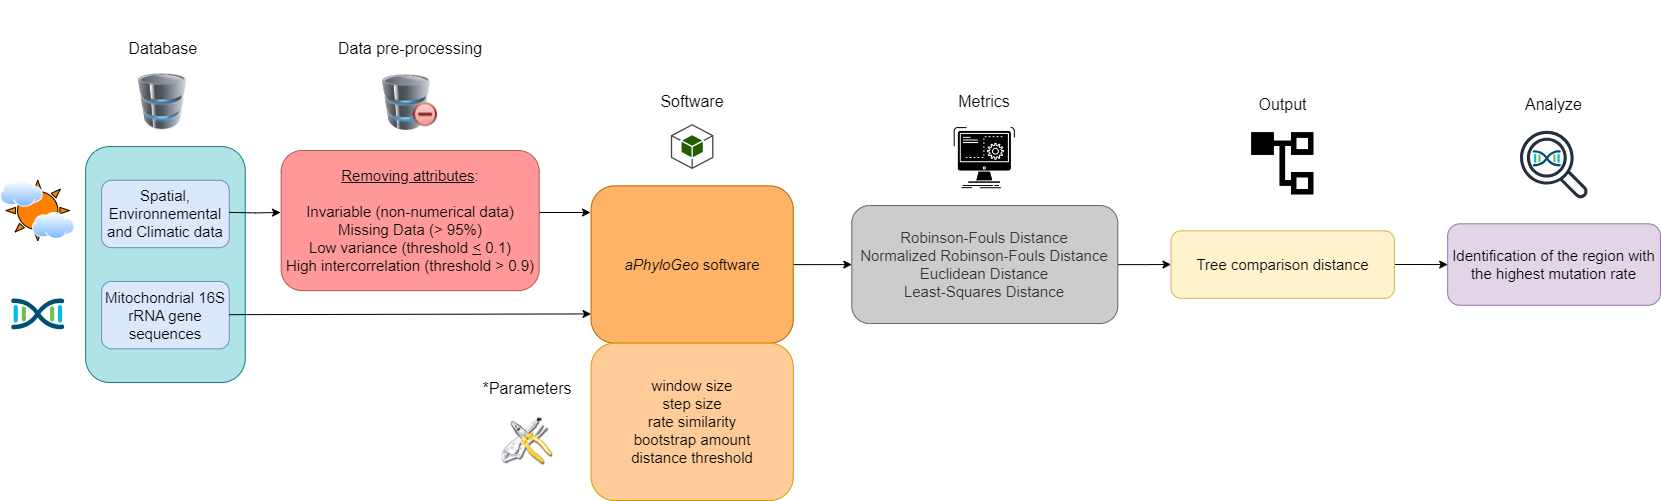
\includegraphics[width=0.7\textwidth]{diagram.drawio.png}
    \caption{Flow chart summarizing the Materials and Methods section workflow. Six different colors highlight the blocks. The first block (blue) represents our database. The second block (red) is data pre-processing, where we remove attributes. The third and fourth blocks (orange) implement the \textit{aPhyloGeo} software and its parameters for our phylogeographic analyses (see in the second step of the \autoref{aPhyloGeo-software}). The fifth block (grey) calculates phylogenetic tree comparison distances. The sixth block (yellow) compares the distances between the phylogenetic and the habitat trees produced. The seventh block (purple) identifies the most divergent habitat parameter(s) of a specific region of the partial sequence of the 16S rRNA mitochondrial gene based on the results of tree comparisons. *See YAML files on \href{https://github.com/tahiri-lab/aPhyloGeo}{GitHub} for more details on these parameters. \label{fig:fig1}}
\end{figure}

\subsection{Description of the data}
The study area was located in a northern region of the North Atlantic, including the Icelandic Sea, the Denmark Strait, and the Norwegian Sea. The specimens examined were collected as part of the IceAGE project (Icelandic marine Animals: Genetic and Ecology; Cruise ship M85/3 in 2011), which focused on the deep continental slopes and abyssal waters around Iceland \citep{meisner_prefacebiodiversity_2018}. The sampling period for the included specimens was from August 30 to September 22, 2011, and they were collected at depths ranging from 316 m to 2568 m. Detailed protocols concerning the sampling plan, sample processing, DNA extraction steps, PCR amplification, sequencing, and aligned DNA sequences are available in \citep{uhlir_adding_2021}.

\subsection{Data preprocessing}
We used data from the article \citep{uhlir_adding_2021}, the IceAGE project, and related data from the BOLDSystem database, as described in \citep{uhlir_adding_2021}. Given these databases' enormous variety of parameters, we applied a selective reduction procedure. Attributes with little or no variability (non-numerical data) were excluded from our study, for which all data were missing and were not linked to genetic sequences or spatial, environmental, and climatic parameters. Out of the 495 available in the IceAGE dataset, we considered 62 specimens for which partial 16S rRNA mitochondrial gene sequences were available.

Next, we calculated the variance ($S^2$) using the $var()$ function in RStudio Desktop 4.3.2 for each of the selected numerical attributes. This step aimed to eliminate attributes with low variation, as they are unlikely to provide essential data for analysis. We set a variance threshold of ≤ 0.1 to exclude uninformative attributes. The latter allows us to retain attributes whose variability is reasonably sufficient for our analyses while rejecting those with little variation. Only water salinity was eliminated based on this criterion ($S^2\textsubscript{Salinity} = 0.02146629$). The formula (see Equation \ref{variance}) and code (\autoref{lst:variance}) used to calculate the variance of our final features, available in the data file on \href{https://github.com/tahiri-lab/Cumacea_aPhyloGeo}{GitHub}, are provided below:

\begin{equation}\label{variance}
    S^2 = \frac{\sum_{i=1}^{n} (x_i - \bar{x})^2}{n-1}
\end{equation}

where $S^2$ is the variance of the attribute, $x_i$ represents each attribute value, $\bar{x}$ is the average of the values for this attribute, and $n$ is the number of values for this attribute in the dataset.

%\autoref{lst:variance}.
\begin{lstlisting}[label=lst:variance,language=R,caption=RStudio script to calculate the variance of each numerical attributes in our final dataset]
# Import data from CSV file
# Read the dataset "Final_Data_Article.csv" and store it in an object called Data.
# The data is read with semicolon (;) as the delimiter.
Data <- read.csv(file = "Final_Data_Article.csv", header = TRUE, sep = ";")

# Calculate the variance of numerical attributes only from the dataset
# This snippet computes the variance for each numerical column.
# Non-numeric columns are excluded from the calculation.
variances <- sapply(Data, function(x) {
  # Check if the column is numeric
  if (is.numeric(x)) {
    # Compute variance, excluding NA values
    var(x, na.rm = TRUE)
  } else {
    NA  # Return NA for non-numeric columns
  }
})

# Display variances
# Print the calculated variances for each numerical attribute.
print(variances)
\end{lstlisting}

To refine our dataset, we calculated the Pearson correlation ($r$) between attributes using the $cor()$ function in RStudio Desktop 4.3.2. Features exhibiting strong correlations with each other (threshold > 0.90) were removed to avoid repetition and guarantee attribute independence. We considered the threshold of > 0.90 to be an adequate compromise between preserving properties for our analyses and eliminating the repetition of information in our data. Since we have three missing data for O\textsubscript{2} concentration (mg/L), we have used the "pairwise.complete.obs method". This method calculates the Pearson correlation matrix using all accessible pairs of observations, even if some data are missing. Using the above threshold, four attributes were discarded: latitude (DD) at the start of sampling (Lat_start_end: $r = 0.9996658$), longitude (DD) at the end of sampling (Long_start_end: $r = 0.9999979$), depth (m) at the end of sampling (Depth_start_end: $r = 0.9998579$) and wind direction at the start of sampling (WindD_start_end: $r = 0.9752331$). The decision to remove these attributes was based on their variance ($S^2$) value: $S^2\textsubscript{Lat_start} = 10.03077$ and $S^2\textsubscript{Lat_end} = 10.71335$; $S^2\textsubscript{Long_start} = 30.47940$ and $S^2\textsubscript{Long_end} = 30.47574$; $S^2\textsubscript{Depth_start} = 776437.1$ and $S^2\textsubscript{Depth_end = 775394.7$; $S^2\textsubscript{WindD_start} = 2.405077$ and $S^2\textsubscript{WindD_end} = 4.482285$. The formula (see Equation \ref{pearson}) and code (\autoref{lst:pearson}) used to calculate the Pearson correlation coefficient between our final numerical attributes are shown below:

\begin{equation}\label{pearson}
    r = \frac{\sum_{i=1}^{n} (x_i - \bar{x})(y_i - \bar{y})}{\sqrt{\sum_{i=1}^{n} (x_i - \bar{x})^2 \sum_{i=1}^{n} (y_i - \bar{y})^2}}
\end{equation}

where $r$ is the Pearson correlation coefficient between two attributes, $x_i$ are the values of an attribute, $y_i$ are the values of another attribute, $\bar{x}$ and $\bar{y}$ are respectively the averages of the two attributes, and $n$ is the sample size of the two attributes.

%\autoref{lst:pearson}.
\begin{lstlisting}[label=lst:pearson,language=R,caption=RStudio script to calculate the Pearson correlation coefficient between all the numerical attributes in our final dataset]
# Import data from the CSV file
# Read the dataset "Final_Data_Article.csv" and store it in an object called Data.
# The data is read with semicolon (;) as the delimiter.
Data <- read.csv(file = "Final_Data_Article.csv", header = TRUE, sep = ";")

# Select numeric columns only from the dataset
# This code filters the dataset to include only numeric columns.
# Create a new dataframe that contains only the columns with numeric data.
numeric_Data <- Data[sapply(Data, is.numeric)]

# Calculate Pearson correlation matrix
# This code calculates the Pearson correlation matrix for the numeric columns.
# The “pairwise.complete.obs” argument ignores missing values.
correlation_matrix <- cor(numeric_Data, use = "pairwise.complete.obs")

# Display correlation matrix
# Print the resulting Pearson correlation matrix.
print(correlation_matrix)
\end{lstlisting}

This selection of attributes and data resulted in a table containing 62 rows ($n=62$) and 16 columns (number of attributes). 

\subsection{Selected attributes in the IceAGE database}

\subsubsection{Geographic data} 

\begin{itemize}
\item The latitude (see Figure \ref{fig:fig2}a) at the end of sampling and longitude (see Figure \ref{fig:fig2}b) at the start of sampling, both in decimal degrees (DD), as they are intimately linked to the environmental gradients and historical mechanisms modeling genetic heterogeneity \citep{gaither2013origins}.
\item The sectors across the seas around Iceland: the Denmark Strait ($n=28$), the Iceland Basin ($n=15$), the Irminger Basin ($n=12$), the Norwegian Sea ($n=4$), and the Norwegian Basin ($n=3$). 
\end{itemize}

\subsubsection{Environmental data} 
\begin{itemize}
\item Depth (m) at the start of sampling (see Figure \ref{fig:fig2}c), as well as water temperature ($^\circ$C) (see Figure \ref{fig:fig2}e), and O\textsubscript{2} concentration (mg/L) (see Figure \ref{fig:fig2}f), as these are vital elements of the marine ecosystem that have an impact on the distribution and evolutionary acclimatization of marine species \citep{rex2006global, danovaro2010first}. 
\item Since the sedimentary characteristics directly influence the distribution of Cumacea \citep{uhlir_adding_2021}, they were included in our data. In this study, they are divided into six ecological niche categories: mud ($n=30$), sandy mud ($n=15$), sand ($n=9$), forams ($n=3$), muddy sand ($n=3$), and gravel ($n=2$).
\end{itemize}

\subsubsection{Climatic data} 
Wind speed (m/s) (see Figure \ref{fig:fig2}d) at the start and end of sampling and wind direction at the end of sampling were also included, giving the contribution of wind to benthic ecosystem dynamics and the restructuring of species distribution by wind currents and sediment transport \citep{siedlecki2016experiments, waga_recent_2020,saeedi_environmental_2022}. The wind direction at the end of sampling comprises eight orientations: south (S, $n=15$), southwest (SW, $n=15$), northeast (NE, $n=9$), west-southwest (WSW, $n=7$), southeast (SE, $n=6$), north-northwest (NNW, $n=5$), south-southeast (SSE, $n=3$), and east (E, $n=2$). 

\subsection{Selected attributes in the BOLDSystem database}
\subsubsection{Taxonomic data} 
The family, genus, and scientific name of the Cumacea sampled were integrated into our data to study evolutionary relationships and genetic variation to habitat attributes among the specimens in our dataset. These comprise seven families: Diastylidae ($n=21$), Lampropidae ($n=13$), Leuconidae ($n=12$), Astacidae ($n=7$), Bodotriidae ($n=4$), Ceratocumatidae ($n=3$), and Pseudocumatidae ($n=2$). A total of 20 Cumacea species were found in our sample (see Figure \ref{fig:fig3}). We have also included the sample identity (id) so that each sample remains unique. Some specimens were only identified to genus ($n=1$) or family ($n=5$).

\subsection{Selected attributes from article \cite{uhlir_adding_2021}} 
\subsubsection{Other environmental data} 
The habitat and water mass of the sampling points were the only water attributes taken directly from Table 1 of \citep{uhlir_adding_2021}, as they can give us insight into how they may affect Cumacea genetic diversity and the acclimatization of these species in the GIN seas around Iceland. Thus, the water masses definitions, as described in \citep{uhlir_adding_2021}, were used as a reference: Arctic Polar Water (APW, $n=15$), Iceland Sea Overflow Water (ISOW, $n=15$), North Atlantic Water (NAW, $n=9$), warm Norwegian Sea Deep Water (NSDWw, $n=8$), Arctic Polar Water/Norwegian Sea Arctic Intermediate Water (APW/NSAIW, $n=7$), Labrador Sea Water (LSW, $n=3$), cold Norwegian Sea Deep Water (NSDWc, $n=3$), and Norwegian Sea Arctic Intermediate Water (NSAIW, $n=2$) (see Figure \ref{fig:fig4}). In terms of habitat, we considered the three categories used in \citep{uhlir_adding_2021}: Deep Sea ($n=38$), Shelf ($n=15$), and Slope ($n=9$) (see Figure \ref{fig:fig5}).

\subsubsection{Genetic data} 
To better understand the relationships between benthic species and their evolutionary responses, genetic data are required \citep{uhlir_adding_2021}. Thus, the aligned partial DNA sequence of the 16S rRNA mitochondrial gene region of each sample was included in our analyses. This region is standard in phylogeny and phylogeography studies \citep{hugenholtz1998impact} and sufficiently conserved over time to guarantee exact alignments between different species or populations \citep{saccone1999evolutionary}. We examined 62 of the 306 aligned DNA sequences used for phylogeographic analyses by \citep{uhlir_adding_2021}. As some specimens in our sample have their DNA sequence duplicated, or even quadruplicated with a difference of one or two nucleotides, we took into account the longest-aligned DNA sequence of each specimen.

\subsection{{\textit{aPhyloGeo} software}\label{aPhyloGeo-software}}
Developed by My-Linh Luu, Georges Marceau, David Beauchemin, and Nadia Tahiri, we used the cross-platform Python software \textit{aPhyloGeo} for our phylogeographic analyses, designed to analyze phylogenetic trees using ecological and geographic attributes (\autoref{lst:main}), enabling us to understand the evolution of species under different environmental conditions \citep{koshkarov_phylogeography_2022}. 

We selected this software for our analysis because, to our knowledge, it is the first phylogeographic tool capable of establishing similarity or dissimilarity between species genetics and environmental, climatic, and geographical attributes \citep{koshkarov_phylogeography_2022} - precisely the objective of our study. The \textit{aPhyloGeo} software offers several key functionalities:

\begin{enumerate}[label=\arabic*.]
\item Phylogenetic tree evaluation: The software elucidates the evolutionary relationships between species based on their genetic sequences, which is essential for interpreting phylogeographic models that link the evolution of species to their spatial distribution and their biological and meteorological context \citep{koshkarov_phylogeography_2022}.
\item Ecological and regional dissimilarity analysis: It enables the detection of divergence and convergence between genetic sequences and habitat attributes. This software property is important for identifying the effect of these attributes on the genetic fluctuations and evolutionary history of these Cumacea species \citep{koshkarov_phylogeography_2022}.
\item Evaluation of genetic diversity: \textit{aPhyloGeo} measures genetic heterogeneity, making it possible to recognize potential evolutionary processes (e.g., mutation, speciation, genetic drift, and selection pressures) and local adaptations.
\end{enumerate}

%\autoref{lst:main}.
\begin{lstlisting}[label=lst:main,language=Python,caption=Main script for tutorial using the aPhyloGeo package.]
# This script outlines the main steps for processing genetic and attribute data using the aPhyloGeo package.
# Install aPhylGeo package
pip install aPhyloGeo

# Install the Poetry package to automatically manage the virtual environment

# Import necessary modules
import pandas as pd
import time
from aphylogeo.alignement import AlignSequences
from aphylogeo.params import Params
from aphylogeo import utils
from aphylogeo.genetic_trees import GeneticTrees
    
if __name__ == "__main__":

    # Load parameters from a configuration file
    # Load parameters necessary for the analysis from a specified file.
    Params.load_from_file()

    # Load the sequence file
    # Loads the genetic sequence file specified by the reference gene filepath.
    sequence_file = utils.loadSequenceFile(Params.reference_gene_filepath)

    # Create an AlignSequences object
    # This object is responsible for aligning the genetic sequences.
    align_sequence = AlignSequences(sequenceFile)

    # Load attribute data from a CSV file
    # This reads the attributes data into a pandas DataFrame.
    attribute_data = pd.read_csv(Params.file_name)

    # Perform the alignment of sequences
    # This method aligns the genetic sequences and stores the results.
    alignments = align_sequence.align()

    # Generate phylogenetic trees based on aligned sequences
    # Create phylogenetic trees from the multiple sequence alignments (MSA).
    genetic_trees = utils.geneticPipeline(alignments.msa)
    
    # Create a GeneticTrees object
    # Represent the generated phylogenetic trees in Newick format.
    trees = GeneticTrees(trees_dict=genetic_trees, format="newick")
   
    # Generate attribute trees based on attribute data
    # Create trees representing the relationships between different attributes.
    attribute_trees = utils.climaticPipeline(attribute_data)
    
    # Filter the results based on the generated trees
    # Filter the results to ensure they meet certain criteria.
    utils.filterResults(attribute_trees, genetic_trees, attribute_data)
\end{lstlisting}

The \textit{aPhyloGeo} Python package is freely and publicly available on \href{https://github.com/tahiri-lab/aPhyloGeo}{GitHub}, and is also available on \href{https://pypi.org/project/aphylogeo/}{PyPi}, to facilitate complex phylogeographic analyses. The software process has three main stages:

\begin{enumerate}
\item \textbf{The first step} was to collect DNA sequences from Cumacea of sufficient quality for the needs of our results \citep{koshkarov_phylogeography_2022}. In this study, 62 Cumacea samples were selected to represent 62 partial sequences of the 16S rRNA mitochondrial gene. We then included, from our database, two climatic attributes, namely wind speed (m/s) at the start and end of the sampling; three environmental characteristics, such as depth (m) at the start of sampling, water temperature ($^\circ$C), and O\textsubscript{2} concentration (mg/L); and two geographic variables, latitude (DD) at the end of sampling and longitude (DD) at the start of sampling.

\item \textbf{In the second step}, trees were generated separately from biological, spatial, meteorological, and genetic data. Concerning spatial attributes, we calculated the dissimilarity between each pair of Cumacea from distinct spatial conditions \citep{koshkarov_phylogeography_2022}. This produced a symmetrical square matrix \citep{koshkarov_phylogeography_2022}. The {neighbor-joining algorithm}\footnote{It is a method used to construct phylogenetic trees using distance matrices.} was used to build the spatial tree from this matrix \citep{koshkarov_phylogeography_2022}. Each geographic attribute gives rise to a tree. If there are $m$ windows affected by this attribute, there will be $m$ geographic trees. The same approach was applied to biological, meteorological, and genetic data. 

For the genetic data, phylogenetic reconstruction was repeated to build genetic trees based on 62 partial sequences of the 16S rRNA mitochondrial gene, considering only data within a window that progresses along the alignment \citep{koshkarov_phylogeography_2022}. This displacement can vary according to the steps and the size of the window defined by the user (their length is determined by the number of base pairs (bp)) \citep{koshkarov_phylogeography_2022}. 

In our case, we set up the \textit{aPhyloGeo} software as follows: $pairwiseAligner$ for sequence alignment; $\text{Hamming distance}$ to measure simple dissimilarities between sequences of identical length; $\text{Wider Fit by elongating with Gap (starAlignment)}$ algorithm takes alignment gaps into account, which is often mandatory in the case of major deletions or insertions in the sequences; $\text{windows\_size}$: 1 nucleotide (nt); and finally, $\text{step\_size}$: 10 nt. The last two configurations imply that for each 1 nt window, a phylogenetic tree is produced using the nucleotide of each Cumacea, then the window is moved by 10 nt, creating a new tree. Each window in the alignment will give a genetic tree. If there are $n$ windows, there will be $n$ phylogenetic trees. Genetic trees will be used in an object called $T_1$, while spatial and ecological trees are used in another object called $T_2$.

\item \textbf{In the third step}, the genetic trees constructed in each sliding window are compared with ecosystemic, atmospheric, and regional trees using Robinson-Foulds distance \citep{robinson_comparison_1981}, normalized Robinson-Foulds distance and Euclidean distance. These contribute to understanding the correspondence between Cumacea genetic sequences and their habitat. The approach also takes bootstrapping into account \citep{koshkarov_phylogeography_2022}. The results of these metrics were obtained using the functions $robinson\_foulds(tree1, tree2)$ and $euclidean\_dist(tree1, tree2)$ from the \textit{aPhyloGeo} software and were organized by the main function (\autoref{lst:main}). Those for the normalized Robinson-Foulds distance were obtained with the function $robinson\_foulds(tree1, tree2)$ (see the last line of code in \autoref{lst:robinsonFoulds}). The metric output tells us which of our attributes has the greatest divergence of phylogenetic relationships in our samples, based on the magnitude of the metric distances (see Figure \ref{fig:fig6} and Figure \ref{fig:fig7}). 

In addition to identifying the specific attribute, a sliding-window approach enables the precise localization of subtle sequences with high rates of genetic mutation \citep{koshkarov_phylogeography_2022}. This method requires shifting a fixed-size window over the alignment of genetic sequences, allowing phylogenetic trees to be reconstructed for each part of the sequence. It therefore allows us to recognize changes in evolutionary relationships along the partial sequence region of the 16S rRNA mitochondrial gene of Cumacea species. This method is essential for determining whether Cumacea-specific gene sequences in this region of their genome may be affected by certain ecological or spatial attributes of their habitat (see Figure \ref{fig:fig6} and Figure \ref{fig:fig7}).
\end{enumerate}

\subsection{Metrics}\label{metrics}
Our phylogeographic study used four distance measures to quantify differences between phylogenetic trees and habitat trees and assess dissimilarities between genetic sequences and our parameters. This enables a comprehensive analysis of the evolutionary dynamics of Cumacea populations in different environmental contexts. 

The following section presents a more concise version of the functions mentioned in the second and third steps of \autoref{aPhyloGeo-software}:

\subsubsection{Robinson-Foulds distance}\label{RF}
The Robinson-Foulds (RF) distance calculates the distance between phylogenetic trees built in each sliding window ($T_1$) and the attributes trees ($T_2$) (see the list in the first step of the \autoref{aPhyloGeo-software}) \citep{tahiri2018new, koshkarov_phylogeography_2022}. This measurement is used to evaluate the topological differences between the two sets of trees (see Equation \eqref{eq:rf} and \autoref{lst:robinsonFoulds}).

For example, it evaluates the number of division differences between phylogenetic trees built within certain user-defined sliding windows (see the second step of the \autoref{aPhyloGeo-software}) and geographic trees built with latitude data (DD) at the end of sampling \citep{robinson_comparison_1981}. A high distance between a specific window and other windows considered in the RF distance analysis may imply that the habitat feature has little to no impact on the evolution of this particular DNA sequence and that the fluctuation of this attribute might not explain the genetic divergences observed.

\begin{equation}\label{eq:rf}
    \text{RF}(T_1, T_2) = | \Sigma(T_1) \Delta \Sigma(T_2) |
\end{equation}

where $\text{RF}(T_1, T_2)$ is the Robinson-Foulds distance between the two sets of trees, $\Sigma(T_1)$ and $\Sigma(T_2)$ are the sets of divisions in trees $T_1$ and $T_2$ and $ \Delta $, the difference between these two sets.

%\autoref{lst:robinsonFoulds}.
\begin{lstlisting}[label=lst:robinsonFoulds,language=Python,caption=Python script for calculating the Robinson-Foulds Distance using the ete3 package in the aPhyloGeo package.]
import ete3

def robinson_foulds(tree1, tree2):
    """
    Calculate the Robinson-Foulds distance between the two sets of trees.

    Parameters:
    - tree1: Genetic trees in Newick format (represent phylogenetic trees in text form).
    - tree2: Ecological and spatial trees in Newick format (represent attributes trees in text form).

    Returns:
    - rf: The Robinson-Foulds distance between the two sets of trees.
    - rf_normalized: The normalized Robinson-Foulds distance.
    """
    # Initialize the Robinson-Foulds distance
    rf = 0

    # Convert trees from Newick format to ete3.Tree objects
    # This parsing allows us to use ete3 methods to compare trees.
    tree1_newick = ete3.Tree(tree1.format("newick"), format=1)
    tree2_newick = ete3.Tree(tree2.format("newick"), format=1)

    # Calculate the Robinson-Foulds distance
    # The method returns RFD, maximum possible RFD, and common leaves (i.e., a taxa) between the trees.
    rf, rf_max, common_leaves = tree1_newick.robinson_foulds(tree2_newick, unrooted_trees=True)

    # If there are no common leaves, set the RFD to 0
    # This makes it possible to deal with cases where the trees have no overlapping taxa.
    if len(common_leaves) == 0:
        rf = 0

    # Return the RFD and its normalized value
    # Normalization is done by dividing RFD by the maximum possible RFD.
    return rf, rf / rf_max
\end{lstlisting}

\subsubsection{Normalized Robinson-Foulds distance}\label{RFnorm}
The normalized Robinson-Foulds (nRF) distance scales the RF distance to account for the size variations in the trees (number of clades; i.e., a group of species with a common origin), allowing a more equitable comparison. It scales the distance to a range between 0 and 1. In our context, the distance has been normalized by $2n-6$, where $n$ represents the number of taxa (see Equation \eqref{eq:rf_norm} and the last line of code in \autoref{lst:robinsonFoulds}). 

Since the size of environmental trees constructed with O\textsubscript{2} concentration data (mg/L) differs from that of other attributes due to missing data, this nRF distance allows us to compare its dissimilarity with the phylogenetic trees in a fairer way \citep{tahiri2018new, koshkarov_phylogeography_2022}. It reveals the relative influence of O\textsubscript{2} concentration (mg/L) on Cumacea phylogenetic relationships, independent of tree size \citep{tahiri2018new, koshkarov_phylogeography_2022}. A high value of this metric between a specific window and other windows considered in the nRF distance analysis suggests that we cannot conclude that there is a correlation between this DNA sequence and the attribute. It may indicate a topological dissimilarity between the habitat attribute tree and the gene trees at that position in the DNA sequence alignments.

\begin{equation}\label{eq:rf_norm}
    \text{RF}_{\text{norm}}(T_1, T_2) = \frac{| \Sigma(T_1) \Delta \Sigma(T_2) |}{| \Sigma(T_1) | + | \Sigma(T_2) |}
\end{equation}

where $ \text{RF}_{\text{norm}}(T_1, T_2)$ is the normalized Robinson-Foulds distance between the two sets of trees, $\Sigma(T_1)$ and $\Sigma(T_2)$ are the sets of divisions in trees $T_1$ and $T_2$ and $ \Delta $, the difference between these two sets.

\subsubsection{Euclidean distance}\label{euclidean}
In our study, the Euclidean distance calculates the distance between two sets of points in a multidimensional space, which designates the divisions of the two sets of trees ($T_1$ and $T_2$). It is used to compare divisions between two respective sets of trees to assess the degree of divergence or similarity of their topologies (see Equation \eqref{eq:euclidean} and \autoref{lst:euclideanDist}). Thus, their distance in the genetic trees and the habitat attribute trees are compared for each pair of leaves.

By comparing the two sets of trees $T_1$ and $T_2$ using this metric, it is possible to measure the extent to which genetic divergences correspond to fluctuations in habitat attributes. This is crucial for interpreting evolutionary relationships with these factors. A high distance of this metric between a specific window and other windows considered in the Euclidean distance analysis suggests evolutionary divergences between members of the Cumacea populations at the level of this DNA sequence and the variation of the habitat attribute (see Figure \ref{fig:fig6}d and Figure \ref{fig:fig7}d). In other words, habitat parameters may not have a dominant contribution to the evolution of this specific sequence of Cumacea populations.

\begin{equation}\label{eq:euclidean}
    d_{\text{Euclidean}}(T_1, T_2) = \sqrt{\sum_{i=1}^{n} (T1_i - T2_i)^2}
\end{equation}

where $ d_{\text{Euclidean}}(T_1, T_2)$ is the Euclidean distance between the two sets of trees, and $T1_i$ and $T2_i$ represent the respective divisions of trees $T_1$ and $T_2$ for each i-th division.

%\autoref{lst:euclideanDist}.
\begin{lstlisting}[label=lst:euclideanDist,language=Python,caption=Python script for calculating the Euclidean distance using the ete3 and the dendropy packages in the aPhyloGeo package]
import ete3
import dendropy

def euclidean_dist(tree1, tree2):
    """
    Calculate the Euclidean distance between the two sets of trees.

    Parameters:
    - tree1: Genetic trees in Newick format (represent phylogenetic trees in text form).
    - tree2: Meteorological, biological, and regional trees in Newick format (represent attributes trees in text form).

    Returns:
    - ed: The Euclidean distance between the two sets of trees.
    """

    # Create a TaxonNamespace object to handle taxon information
    tns = dendropy.TaxonNamespace()

    # Load the first tree from Newick format into a dendropy Tree object
    # Analyzes the string formatted by Newick and prepares the tree for comparison.
    tree1_tc = dendropy.Tree.get(
        data=tree1.format("newick"), 
        schema="newick", 
        taxon_namespace=tns
    )
    
    # Load the second tree from Newick format into a dendropy Tree object
    # Similar to the first tree, this step prepares the second tree for comparison.
    tree2_tc = dendropy.Tree.get(
        data=tree2.format("newick"), 
        schema="newick", 
        taxon_namespace=tns
    )

    # Encode the bipartitions of both trees
    # This step converts the trees into a format where the presence or absence of 
    # Each bipartition (split) is coded, which is necessary to calculate distances.
    tree1_tc.encode_bipartitions()
    tree2_tc.encode_bipartitions()

    # Calculate the Euclidean distance between the two trees
    # The distance is computed based on the differences in the encoded bipartitions.
    ed = dendropy.calculate.treecompare.euclidean_distance(tree1_tc, tree2_tc)

    return ed
\end{lstlisting}

Interestingly, Euclidean distance is more sensitive to the subtle tree topology, making it suitable for identifying detailed correlations between genetic fluctuations and those of habitat parameters \citep{czarna2006topology}. It can therefore be used to study fine divergences between trees, enabling nuanced identification of the effects of habitat attributes on the genetic structure of species \citep{czarna2006topology}. As for the Robinson-Foulds distance (normalized or not), although widely applied in evolutionary biology, it is less sensitive to slight topological dissimilarities, making it less accurate for identifying fine correlations between genetics and habitat parameters due to its structural nature \citep{smith2019bayesian, smith2020information}.

\subsection{Creating Figures}\label{Figures}
Figure \ref{fig:fig2}, Figure \ref{fig:fig3}, Figure \ref{fig:fig6} and Figure \ref{fig:fig7} were made with Python 3.11, while Figure \ref{fig:fig4} and Figure \ref{fig:fig5} were made with RStudio Desktop 4.3.2.

\section{Results}\label{results}
The violin diagrams shown in Figure \ref{fig:fig2} are used to display summary statistics similar to box plots, showing medians (white lines), interquartile ranges (thickened black bars), and the rest of the distributions (thin black lines), except the ``extreme'' points. Wider areas indicate a greater probability of the attributes taking a given value. They summarize the distribution of spatial (latitude at the end of sampling and longitude at the start of sampling, both in DD), atmospheric (wind speed (m/s) at the start of sampling), and ecosystemic (depth (m) at the start of sampling, water temperature ($^\circ$C), and O\textsubscript{2} concentration (mg/L)) data. These diagrams are essential for understanding habitat conditions and highlighting attributes that can potentially influence the genetic adaptability of Cumacea. In Table \ref{fig:tab1} and Figure \ref{fig:fig2}, the parameters are designated by their names from the IceAGE database, except for latitude (DD) at the end of sampling and longitude (DD) at the start of sampling, for which the term ``dec'' has been removed at the end to avoid confusion.

\begin{table}[H]
    \centering
    \caption{Table summarizing key statistics such as mean, median, standard deviation (Std Dev), 1st quartile (Q\textsubscript{1}) and 3rd quartile (Q\textsubscript{3}) of biological (depth (m) at the start of sampling, water temperature ($^\circ$C), and O\textsubscript{2} concentration (mg/L)), spatial (latitude (DD) at the end of sampling and longitude (DD) at the start of sampling) and atmospheric (wind speed (m/s) at the start and end of sampling) attributes for our phylogeographic analyses. \label{fig:tab1}}
    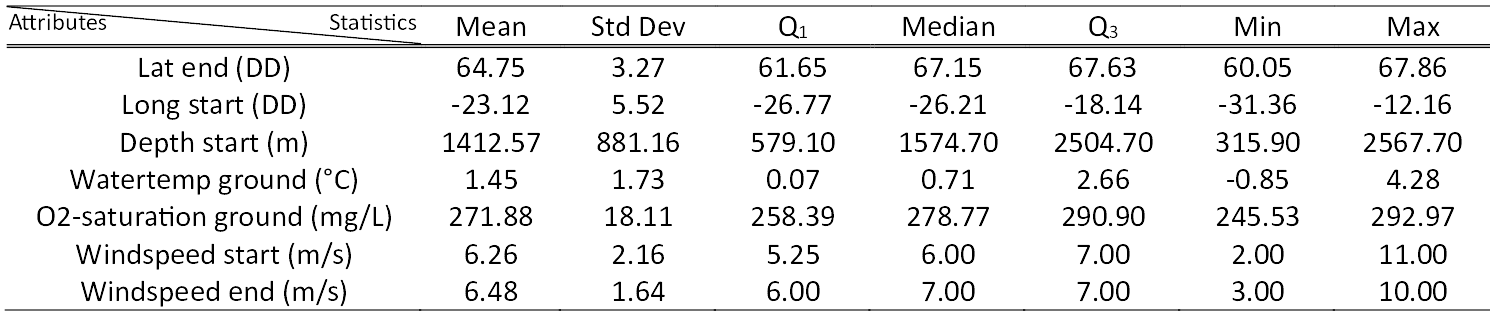
\includegraphics[width=0.7\textwidth]{Table_Attributes_Data.png}
\end{table}

\begin{figure}[htbp]
    \centering
    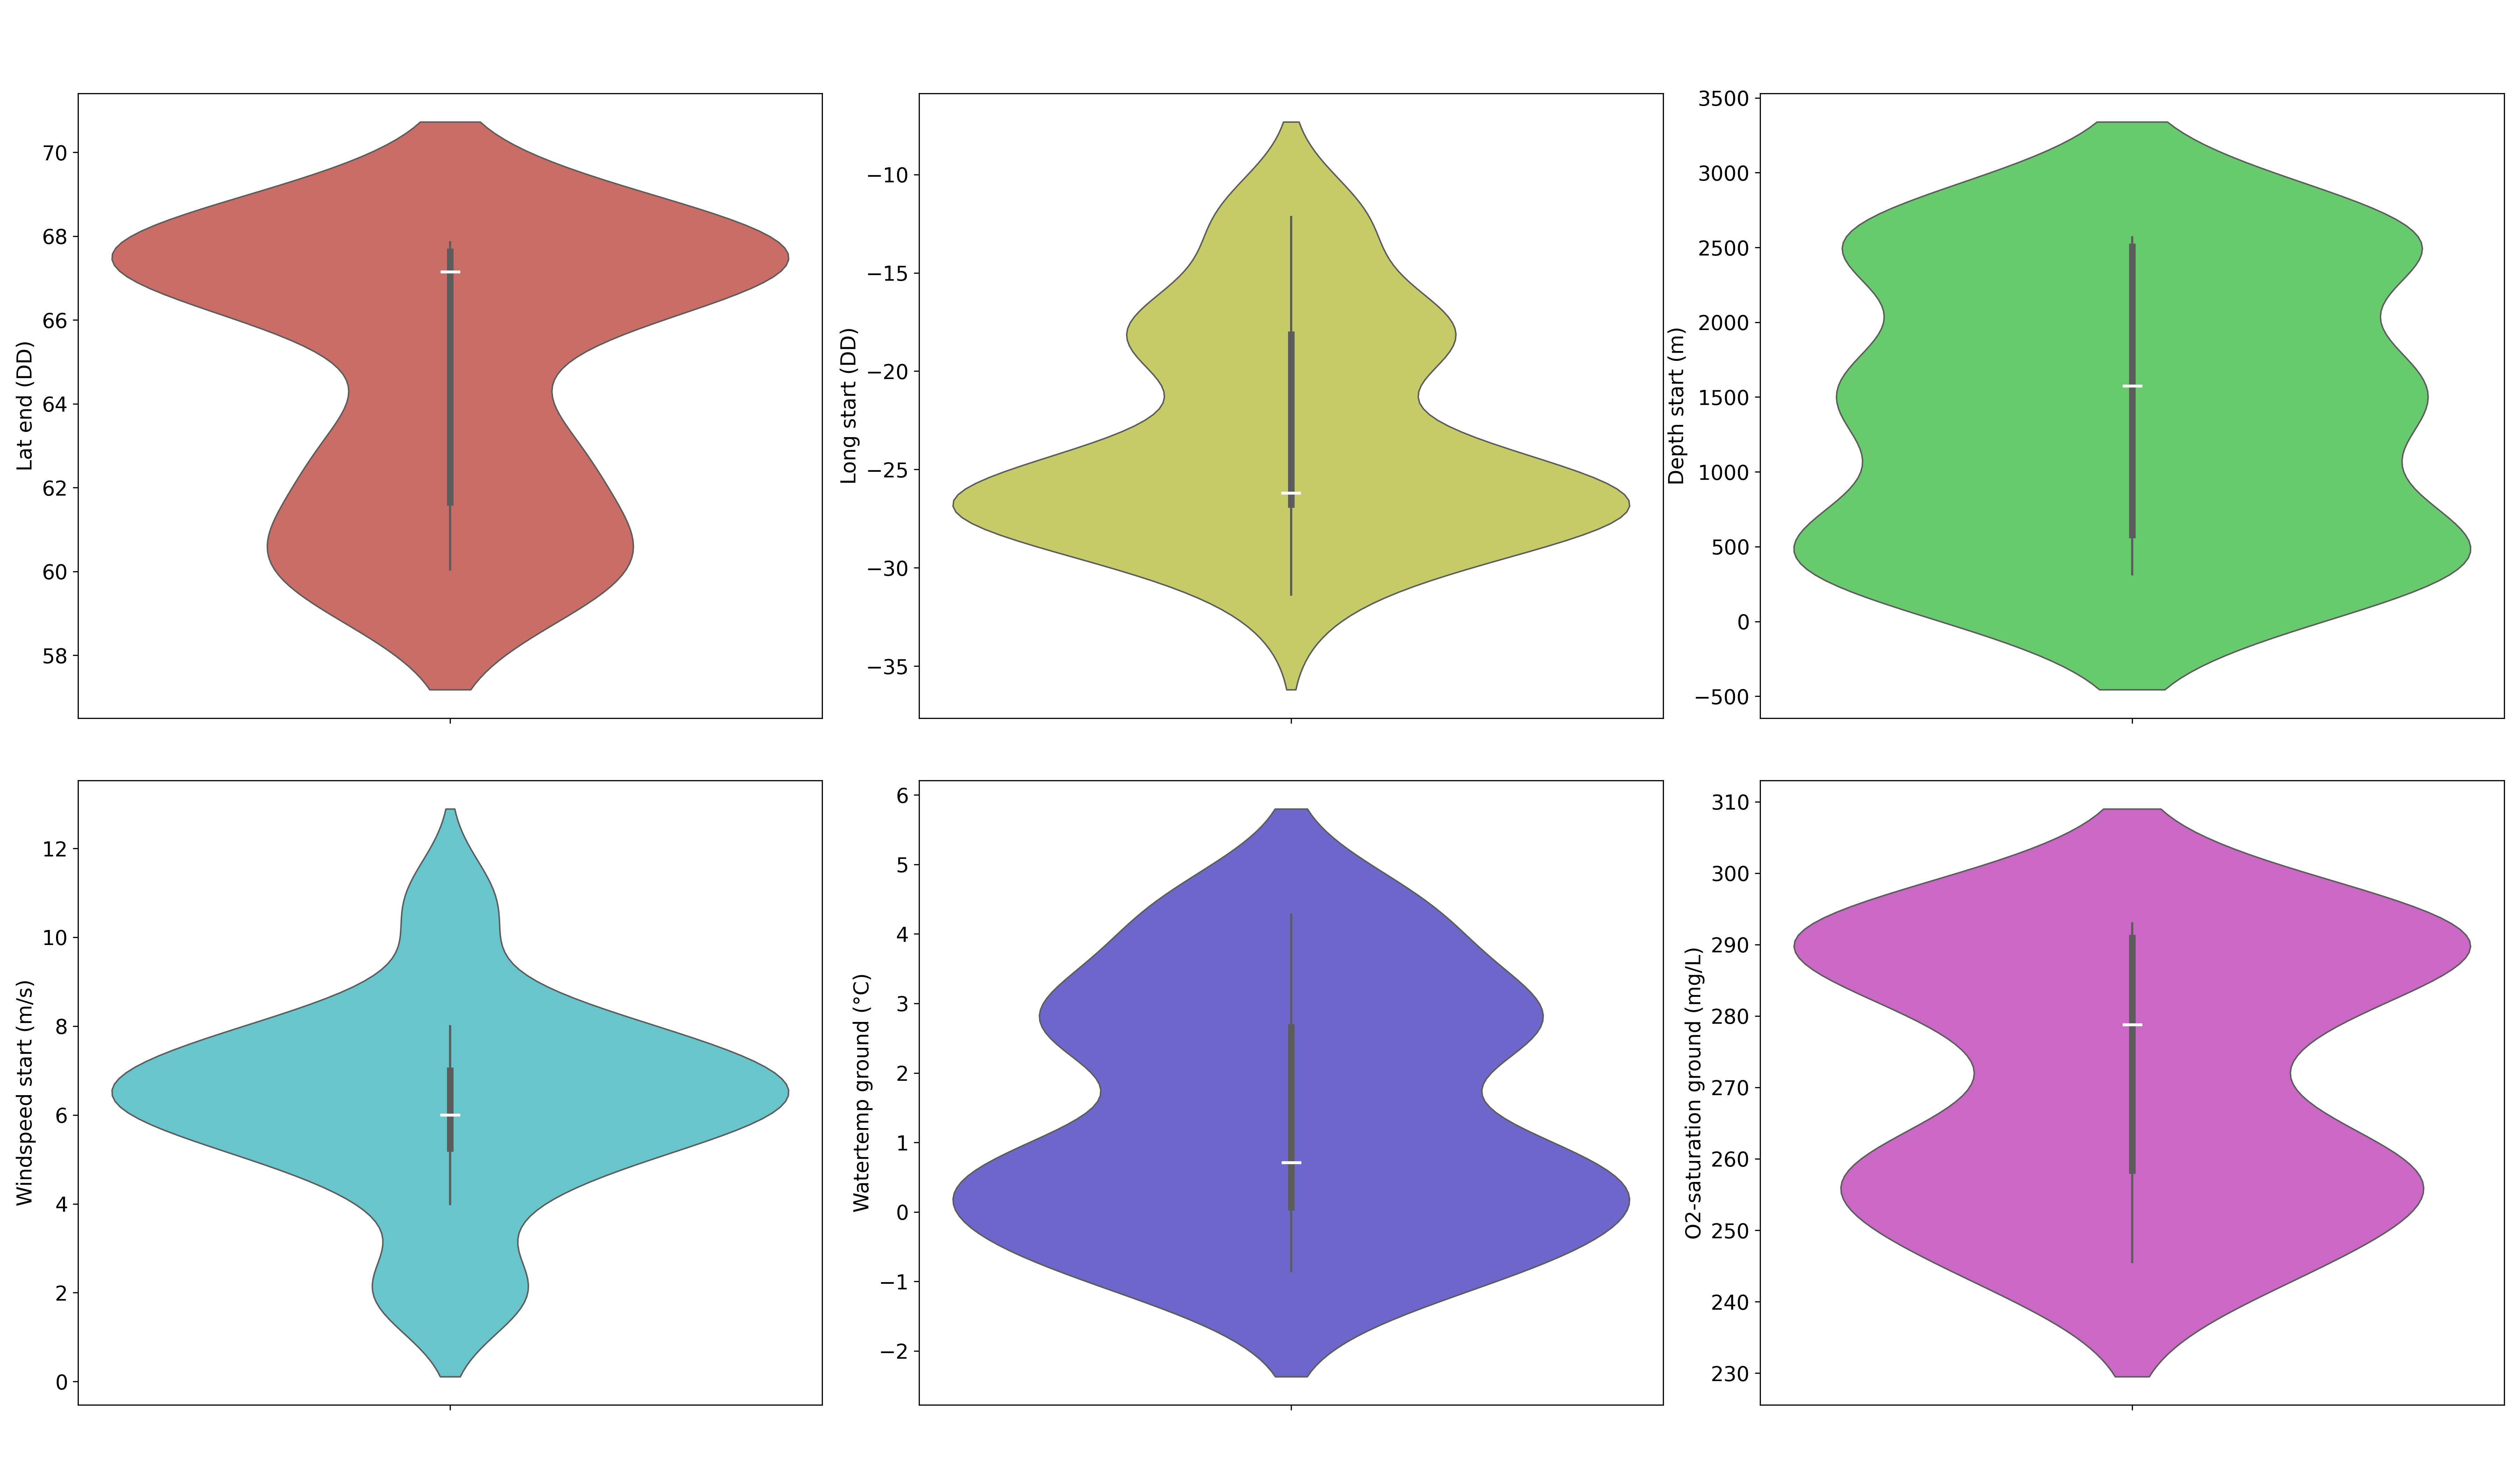
\includegraphics[width=0.7\textwidth]{figure1.jpg}
    \caption{Violin diagrams of two regional attributes, one atmospheric attribute, and three ecosystemic attributes from our sample that provide essential information about the ecological and meteorological conditions of Cumacea habitats. a) Latitude (DD) at the end of sampling (red) suggest that the samples come from two dominant latitudinal (DD) regions (around 61.64 DD and 67.64 DD); b) Longitude (DD) at the start of sampling (yellow) implies that the samples come from two dominant longitudinal (DD) regions (around -26.77 DD and -18.14 DD); c) Depth (m) at the start of sampling (green) suggest that the samples were mainly collected and concentrated at three different depths (m) (around 500 m, 1500 m and 2500 m); d) Wind speed (m/s) at start of sampling (light blue) indicate stable the wind conditions (m/s) at the start of sampling (around 6.00 m/s); e) Water temperature ($^\circ$C) (dark blue) suggest that the samples were mostly collected and concentrated at two different water temperatures ($^\circ$C) (around 0.07 $^\circ$C and 2.66 $^\circ$C); f) O\textsubscript{2} concentration (mg/L) (pink) implies that the samples were primarily collected and concentrated at two different O\textsubscript{2} concentrations (mg/L) (around 258.39 mg/L and 290.90 mg/L). \label{fig:fig2}}
\end{figure}

Our results revealed variability in most habitat attributes, as shown in Figure \ref{fig:fig2}. For instance, the median of the latitude at the end of sampling (67.15 DD; Table \ref{fig:tab1}) is higher than the mean (64.75 DD; Table \ref{fig:tab1}), showing an asymmetric distribution skewed towards lower values. This trend is also observed for depth (m) at the start of sampling (Median: 1574.70 m; Mean: 1412.57 m; see Figure \ref{fig:fig2}c and Table \ref{fig:tab1}) and O\textsubscript{2} concentration (mg/L) (Median: 278.77 mg/L; Mean: 271.88 mg/L; see Figure \ref{fig:fig2}f and Table \ref{fig:tab1}). The bimodal shape of the latitude distribution curve suggests that samples came from two dominant latitudinal regions at the end of sampling (around 61.65 DD and 67.63 DD; see Figure \ref{fig:fig2}a and Table \ref{fig:tab1}). This bimodality is also observed in longitude (DD) at the start of sampling (around -26.77 DD and -18.14 DD; see Figure \ref{fig:fig2}b and Table \ref{fig:tab1}), as well as for water temperature ($^\circ$C) (around 0.07 $^\circ$C and 2.66 $^\circ$C; see Figure \ref{fig:fig2}e and Table \ref{fig:tab1}), and O\textsubscript{2} concentration (mg/L) (around 258.39 mg/L and 290.90 mg/L; see Figure \ref{fig:fig2}f and Table \ref{fig:tab1}).

The median of the longitude (DD) at the start of sampling (-26.21 DD; Table \ref{fig:tab1}) is lower than the mean (-23.12 DD; Table \ref{fig:tab1}), indicating asymmetry on the higher sides (see Figure \ref{fig:fig2}b), as does the water temperature ($^\circ$C) (Mean: 1.45 $^\circ$C; Median: 0.71 $^\circ$C; see Figure \ref{fig:fig2}e and Table \ref{fig:tab1}). Unlike all the other diagrams in Figure \ref{fig:fig2}, the curve of the depth (m) at the start of sampling (see Figure \ref{fig:fig2}c) has a multimodal shape with three prominent peaks, suggesting that the samples were mainly collected and concentrated at three different depths (around 500 m, 1500 m and 2500 m; see Figure \ref{fig:fig2}c).

The mean (6.26 m/s; Table \ref{fig:tab1}) and median of wind speed (m/s) at the start of sampling are fairly similar, with a high density of data around the median (6.00 m/s; see Figure \ref{fig:fig2}d and Table \ref{fig:tab1}). This suggests stable wind conditions (m/s) at the start of sampling. The standard deviation of water temperature ($^\circ$C) is relatively high (1.73 $^\circ$C; Table \ref{fig:tab1}) compared to the mean (1.45 $^\circ$C; Table \ref{fig:tab1}), suggesting acclimatization of Cumacea to a variety of habitat temperatures (-0.851 $^\circ$C – 4.28 $^\circ$C; see Figure \ref{fig:fig2}e and Table \ref{fig:tab1}). The range of data for O\textsubscript{2} concentration (mg/L) shows some variability (245.53 mg/L – 292.97 mg/L; see Figure \ref{fig:fig2}f and Table \ref{fig:tab1}) in the environmental conditions. This reflects a diversity of requirements in terms of O\textsubscript{2} concentration (mg/L), with Cumacea potentially affected by the heterogeneity of biogeochemical cycles, such as photosynthesis, respiration, and organic decomposition, which affect depth-dependent dissolved O\textsubscript{2} concentration (mg/L).

\begin{figure}[htbp]
    \centering
    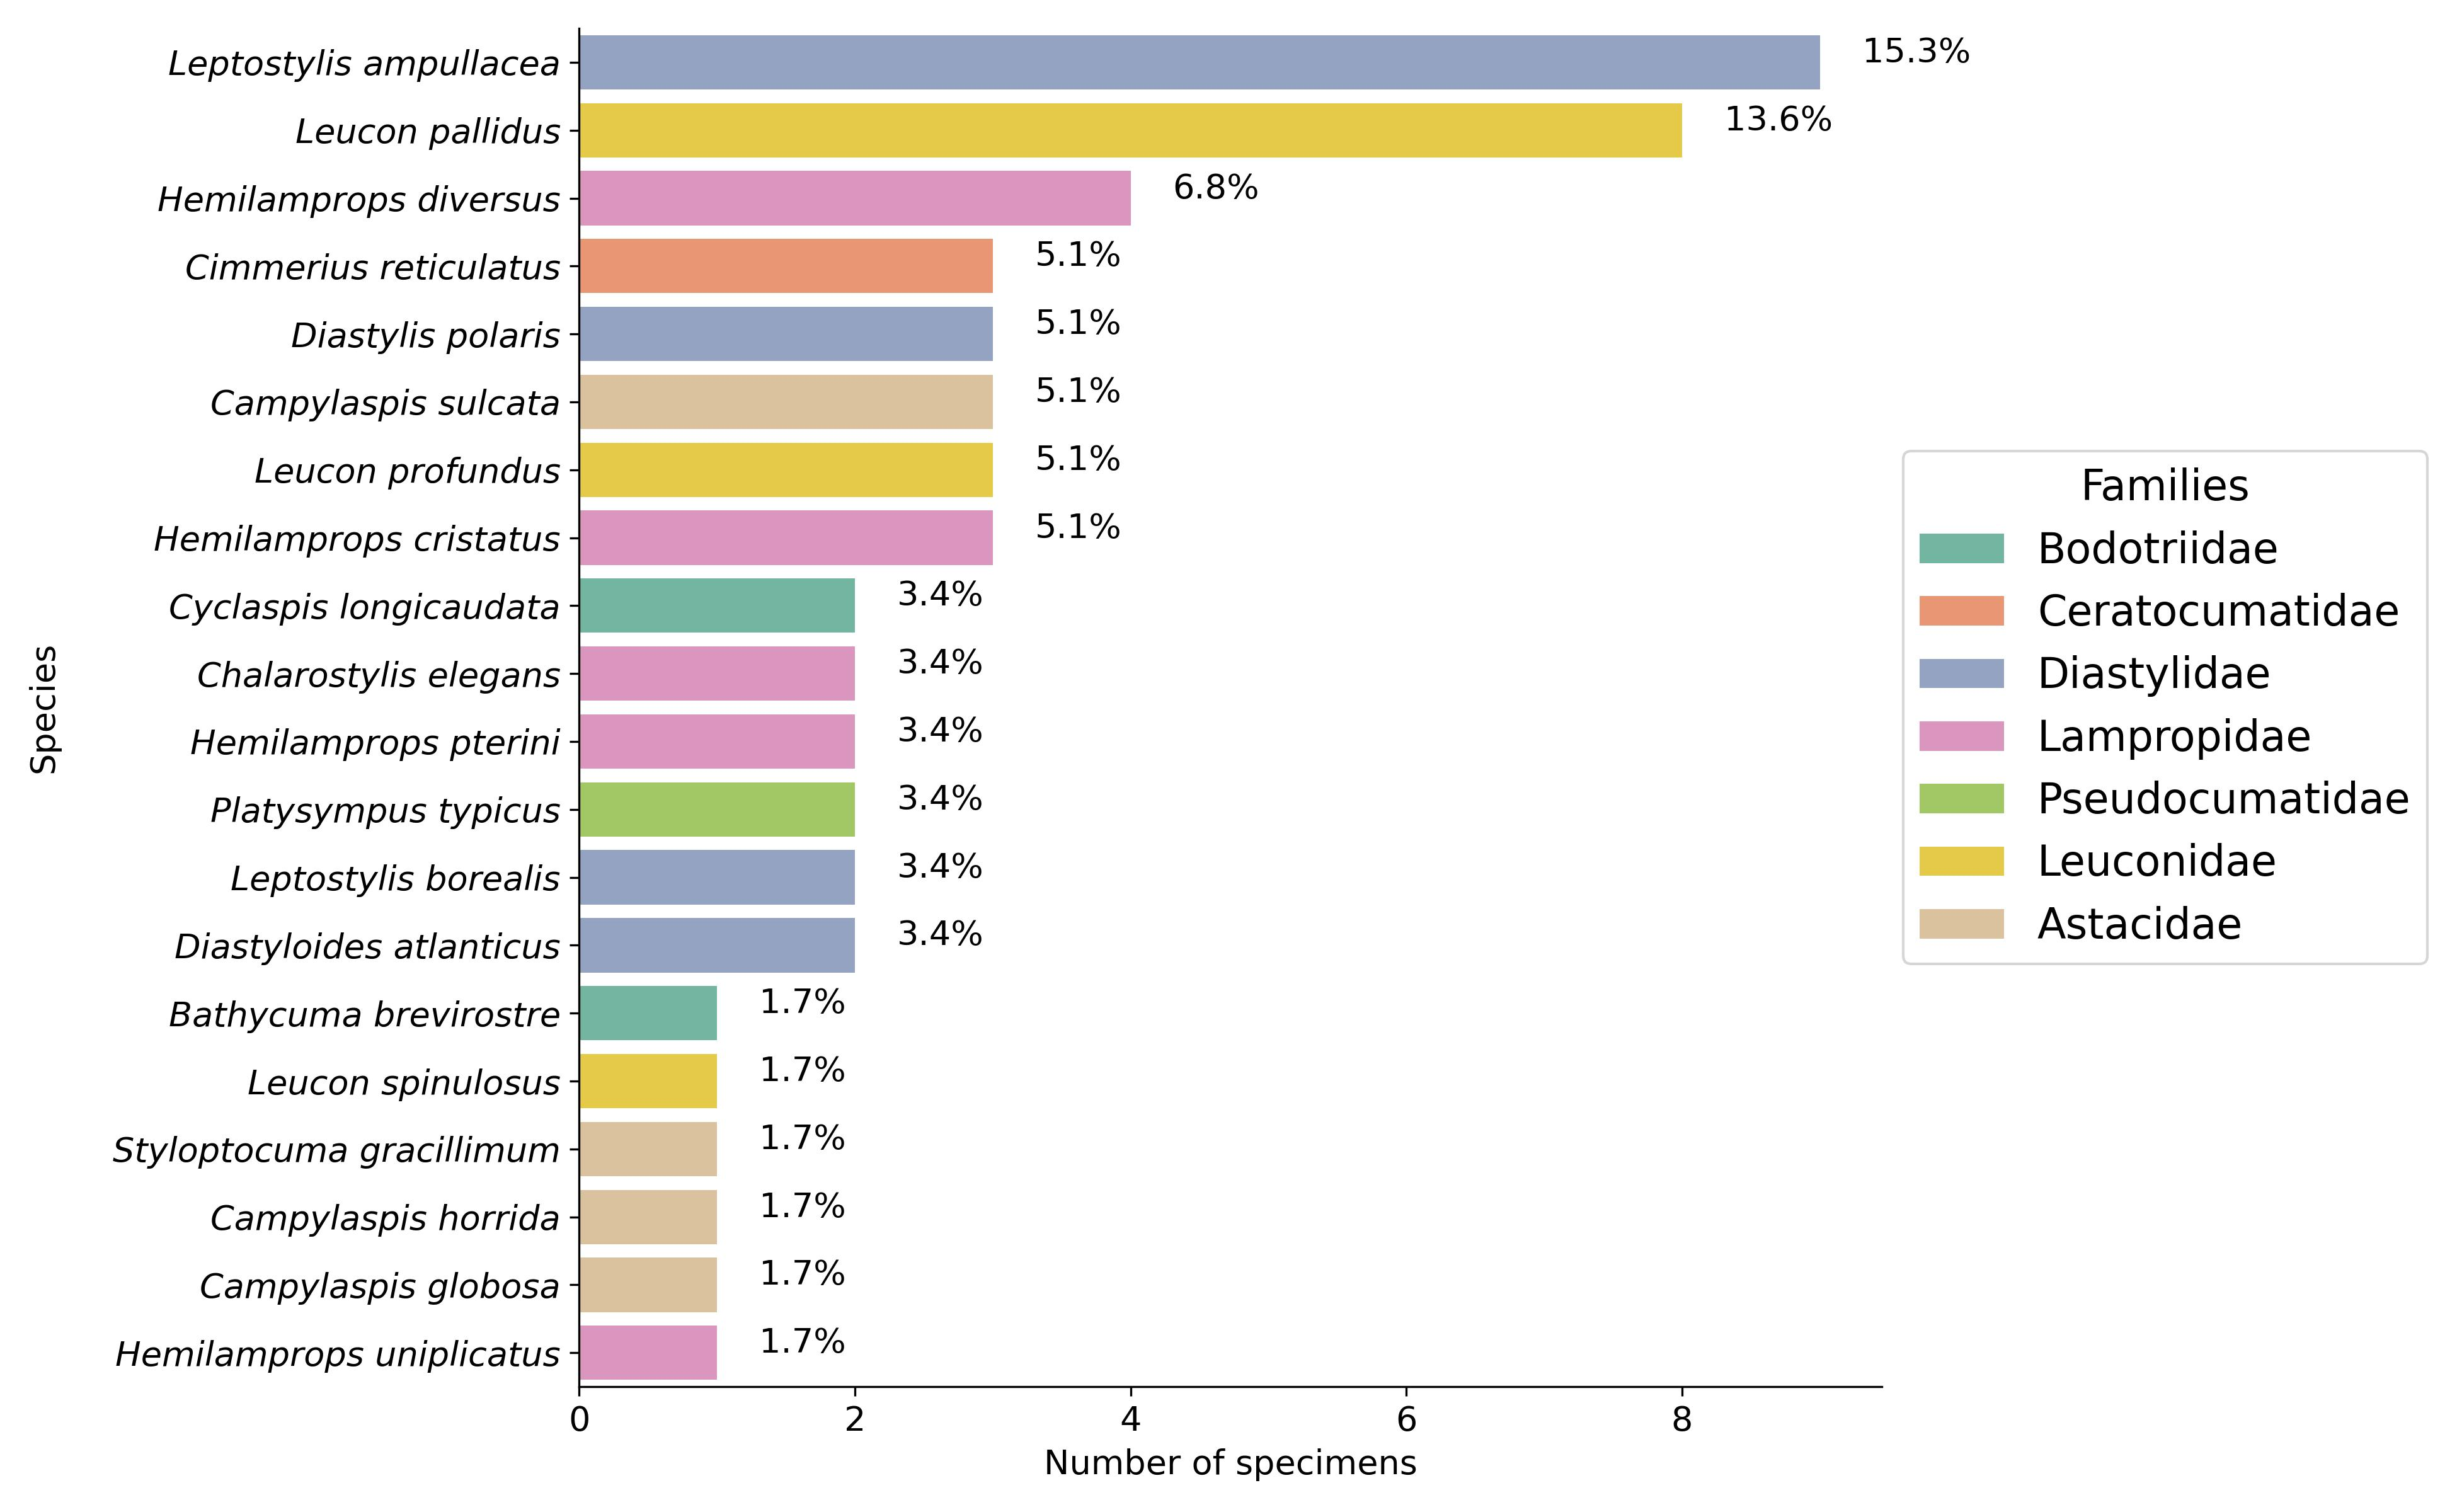
\includegraphics[width=0.7\textwidth]{figure2.jpg}
    \caption{Frequency distribution of Cumacea species in our sample. The bars represent the number of individuals for each species. The percentages (\%) displayed above the bars indicate the relative abundance of each species in the total sample. The mean and median values of the frequency distribution are shown in the top right-hand corner of the histogram. Unlike less common species, those that are abundant (such as \emph{Leptostylis ampullacea} and \emph{Leucon pallidus}) may have adaptive characteristics that enable them to exploit resources more easily, resist interspecific competition or withstand changing biological conditions. \label{fig:fig3}}
\end{figure}

The distribution and diversity of the various Cumacea species found in our sample are shown in Figure \ref{fig:fig3}. It shows that the most represented species are \emph{Leptostylis ampullacea} (14.1\%) and \emph{Leucon pallidus} (12.5\%). In contrast, species like \emph{Bathycuma brevirostre} and \emph{Styloptocuma gracillimum} are less represented (1.6\%), implying that some species may have restricted ecological niches or face ecological forces that limit their distribution. The dominance of certain species (such as \emph{Leptostylis ampullacea} and \emph{Leucon pallidus}) suggests that they may have adaptive traits that enable them to make the most of the accessible resources, resist interspecific competition, or survive in fluctuating ecosystemic conditions, aligns with our study’s aim of relating genetic adaptation to habitat characteristics. 

\begin{figure}[htbp]
    \centering
    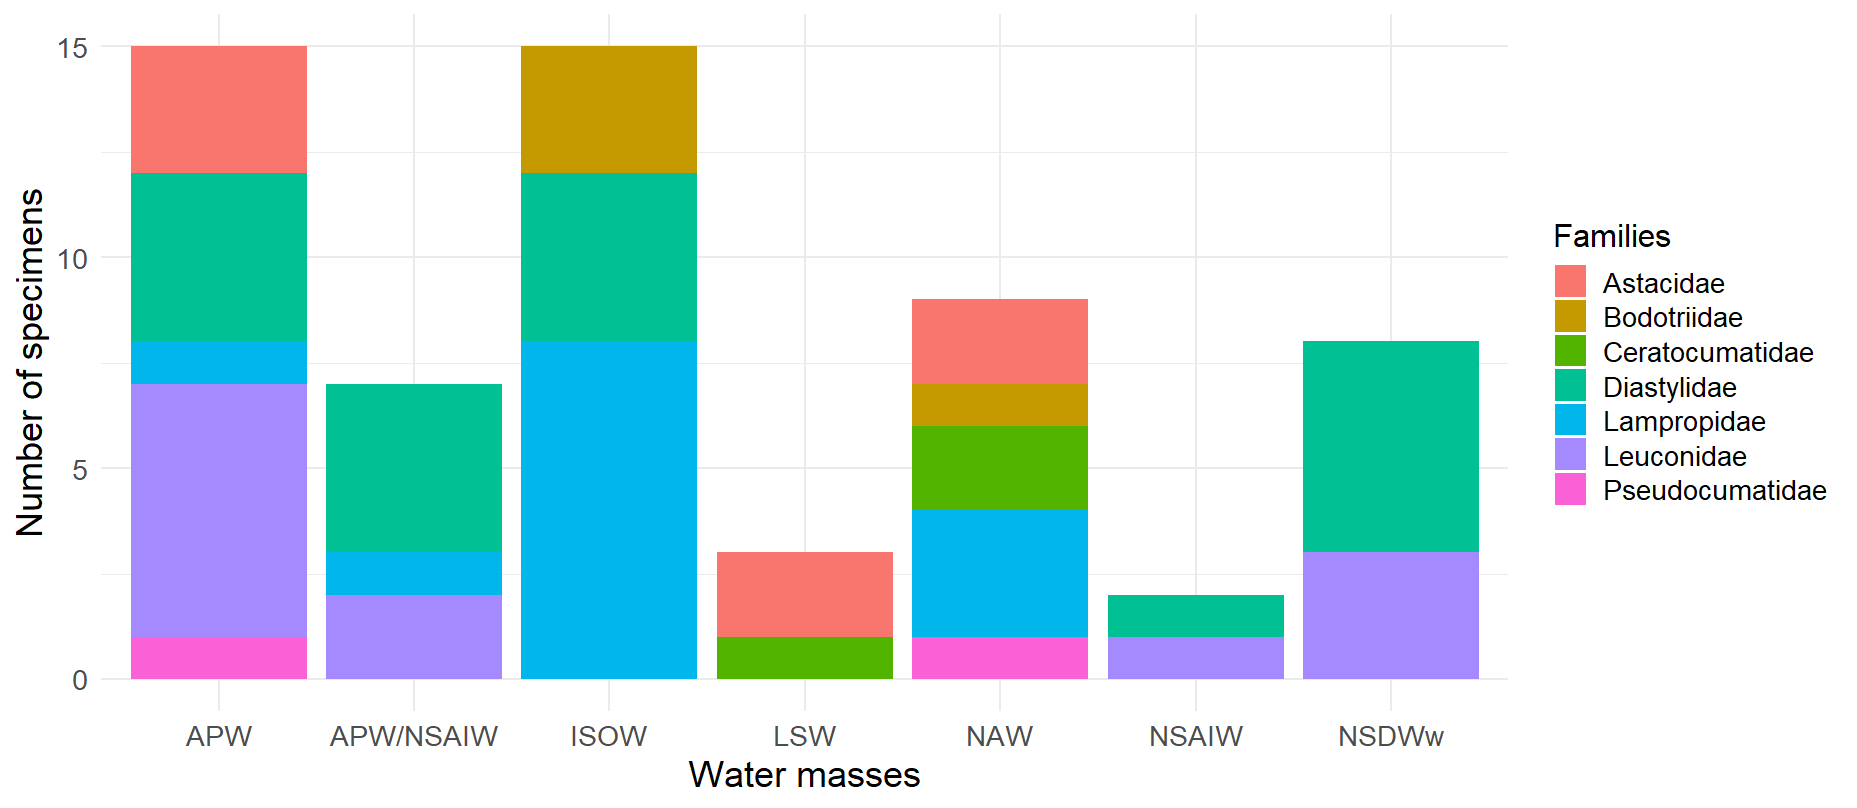
\includegraphics[width=0.7\textwidth]{figure3.png}
    \caption{Distribution of Cumacea families by water mass. This histogram represents the frequency of occurrence of the different Cumacea families in our samples, classified according to the water mass in which they were collected. Eight water mass categories are represented: Arctic Polar Water (APW), Arctic Polar Water/North Sub-Arctic Intermediate Water (APW/NSAIW), Iceland Scotland Overflow Water (ISOW), Labrador Sea Water (LSW), North Atlantic Water (NAW), North Sub-Arctic Intermediate Water (NSAIW), cold North Sub-Atlantic Deep Water (NSDWc), and warm North Sub-Atlantic Deep Water (NSDWw). Seven families are represented: Astacidae (red), Bodotriidae (brown), Ceratocumatidae (green), Diastylidae (turquoise), Lampropidae (blue), Leuconidae (purple), and Pseudocumatidae (pink). The presence of the Diastylidae (turquoise) family in the majority of water bodies (APW, APW/NSAIW, ISOW, NSAIW, NSDWc, and NSDWw) accentuates the resilience and ecological acclimatization of this family to various ecological niches and conditions. \label{fig:fig4}}
\end{figure}

The following figure supports the objective of our study by showing the distribution of the various Cumacea families in the different water bodies (see Figure \ref{fig:fig4}). The Diastylidae family, for example, is the most common in all water bodies (turquoise color in Figure \ref{fig:fig4}), testifying to its resilience and ecological adaptability to a wide variety of habitat conditions, reminiscent of the dominance of \emph{Leptostylis ampullacea} (see Figure \ref{fig:fig3}, 14.1\%) which belongs to the Diastylidae family. 

\begin{figure}[]
    \centering
    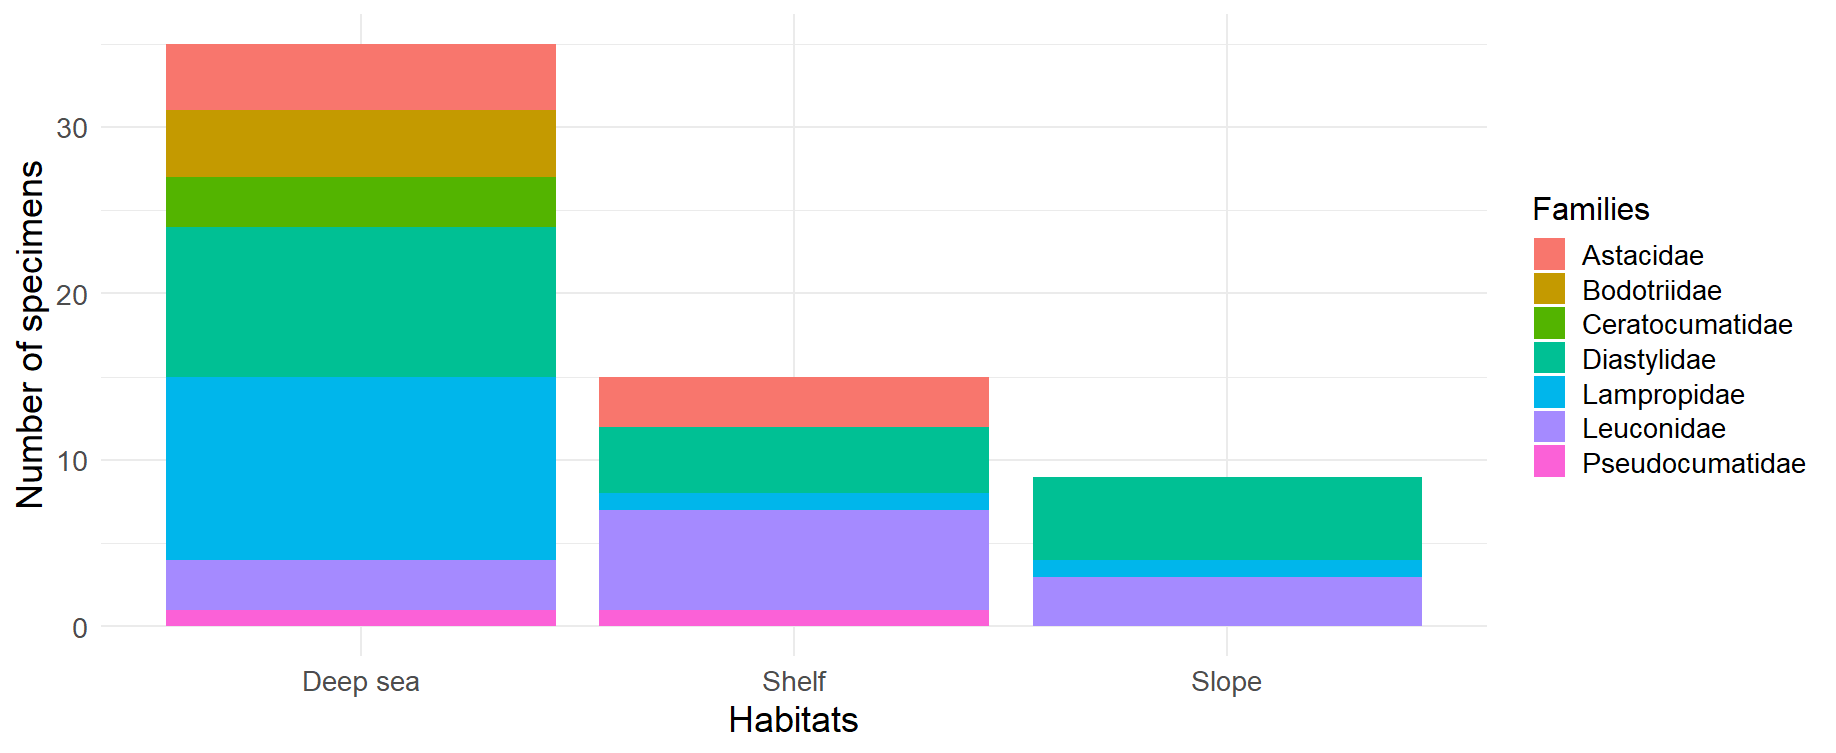
\includegraphics[width=0.7\textwidth]{figure4.png}
    \caption{Distribution of Cumacea families by habitat. This histogram represents the frequency of occurrence of the different Cumacea families in our samples, classified according to the habitat in which they were collected. Three habitat categories are represented: Deep Sea, Shelf, and Slope. Seven families are represented: Astacidae (red), Bodotriidae (brown), Ceratocumatidae (green), Diastylidae (turquoise), Lampropidae (blue), Leuconidae (purple), and Pseudocumatidae (pink). The presence of Cumacea families in more than one habitat, such as Diastylidae (turquoise), Lampropidae (blue), and Leuconidae (purple), may indicate the development of adaptations, whether morphological, physiological, or behavioral, that could favor their persistence in these habitats. \label{fig:fig5}}
\end{figure}

The distribution of samples of the different Cumacea families according to the type of habitat where they were collected during sampling is shown in Figure \ref{fig:fig5}. The deep-sea habitats show the greatest diversity of families, mainly Diastylidae and Lampropidae, suggesting they are well acclimatized to deep-sea conditions. In contrast, the slope has the lowest diversity, with Diastylidae again the most dominant, implying that some Cumacea species have fewer ecological niches or are less adapted to this habitat. Although less diverse than the deep sea, the shelf is dominated by Leuconidae, indicating that this family may be specifically well-acclimated to shelf habitat. These patterns imply that certain Cumacea families, such as the Diastylidae, Lampropidae, and Leuconidae, have developed distinct adaptations (physiological, behavioral, or morphological) to remain in particular ecological niches, reflecting the impact of habitat conditions on the genetic distribution of Cumacea.

\begin{figure}[]
    \centering
    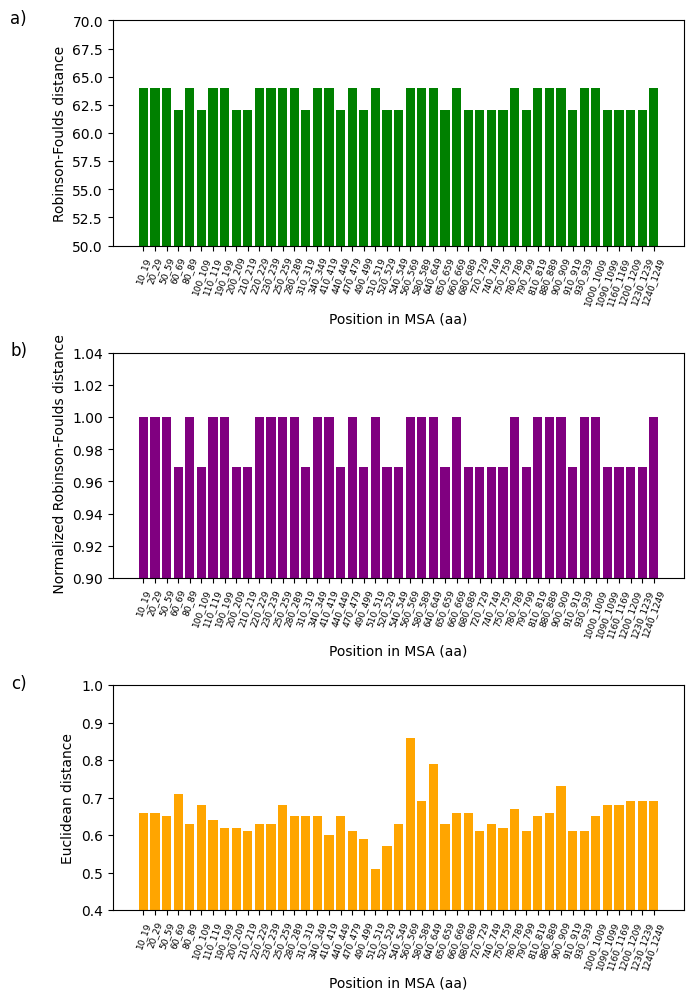
\includegraphics[width=0.7\textwidth]{figure5.png}
     \caption{Analysis of fluctuations in four distance metrics using multiple sequence alignment (MSA): a) Robinson-Foulds distance, b) normalized Robinson-Foulds distance, and c) Euclidean distance. Distance variations are studied to establish the potential dissimilarity between the partial sequence of the 16S rRNA mitochondrial gene of 62 Cumacea specimens and the variability of wind speed (m/s) at the start of sampling. \label{fig:fig6}}
\end{figure}

\begin{figure}[]
    \centering
    
\includegraphics[width=0.7\textwidth]{figure6.png}
    \caption{Analysis of fluctuations in four distance metrics using multiple sequence alignment (MSA): a) Robinson-Foulds distance, b) normalized Robinson-Foulds distance, and c) Euclidean distance. These distances aim to determine the degree of dissimilarity between the partial sequence of the 16S rRNA mitochondrial gene of 62 Cumacea specimens and the variation in O\textsubscript{2} concentration (mg/L) at the sampling sites. \label{fig:fig7}}
\end{figure}

The divergence between the genetic sequences and two attributes, one climatic (wind speed (m/s) at the start of sampling) and the other environmental (O\textsubscript{2} concentration (mg/L)) is presented in Figure \ref{fig:fig6} and Figure \ref{fig:fig7}. All the attributes given in the first step of the \autoref{aPhyloGeo-software} section were analyzed and their script and figure will be soon available in the $img$ and $script$ python file on \href{https://github.com/tahiri-lab/Cumacea_aPhyloGeo}{GitHub}. However, only these two attributes showed the most interesting mutation rate. Using the four metrics mentioned in the \autoref{metrics}, we noticed that the Euclidean distance is particularly sensitive to our data, manifesting considerable sequence variation at the position in MSA 560-569 amino acids (aa) (Euclidean distance: 0.86; see Figure \ref{fig:fig6}d) and 1210-1219 aa (Euclidean distance: 1.23; see Figure \ref{fig:fig7}d). Unlike the other windows for this metric in the two figures (see Figure \ref{fig:fig6}d and Figure \ref{fig:fig7}d), the fluctuations in wind speed (m/s) at the start of sampling and in O\textsubscript{2} concentration (mg/L) do not appear to explain the variations in these two specific sequences. This could indicate the absence of directional selection in these sequences due to these habitat attributes, local selective pressures not considered in our analysis, or other evolutionary factors (e.g., genetic drift or biotic interactions) predominate over these two parameters concerning these two sequences. On the other hand, this may suggest that these two attributes could potentially influence the divergent (i.e., genetic diversification) rather than a convergent adaptation of these Cumacea, reflecting unique evolutionary responses to these specific ecological pressures. These results are consistent with the aim of our study, which is to identify the Cumacea genetic region that diverges most as a function of habitat attribute, to determine whether this is due to divergent local adaptation or other evolutionary processes.

These results provide important insight into the genetic adaptation of Cumacea to their environment. These results need to be analyzed in greater depth to certify their involvement, especially in contrast with \citep{uhlir_adding_2021}, which investigated similar topics of environmental and climatic effects on Cumacea distribution and genetics. The \textit{aPhyloGeo} package is still in the process of being updated.

\section{Conclusion}\label{conclusion}
This study examines the effects of meteorological, regional, and ecosystemic attributes on the genetics of Cumacea in the waters surrounding Iceland. Our main objective is to determine whether there is a discrepancy between the precise genetic information of the partial 16S rRNA mitochondrial gene sequence (i.e. a window) of Cumacea species and their habitat attributes. In addition to data distribution representations (see Figure \ref{fig:fig2}, Figure \ref{fig:fig3}, Figure \ref{fig:fig4} and Figure \ref{fig:fig5}), DNA sequence analyses have identified specific genetic windows that diverge from atmospheric and biological attributes such as wind speed (m/s) at the start of sampling (Position in MSA: 560-569 aa; Euclidean distance: 0.86; see Figure \ref{fig:fig6}d) and O\textsubscript{2} concentration (mg/L) (Position in MSA: 1210-1219 aa; Euclidean distance: 1.23; see Figure \ref{fig:fig7}d). These results may imply our sample may have been shaped by these unique local environments, resulting in genetic sequences adapted to their distinctive conditions.

The novelty in our research lies in the exhaustive divergence between habitat attributes and genetic mutability in Cumacea, particularly in identifying genetic windows associated with habitat fluctuations, which has not been widely investigated in previous studies \citep{manel2003landscape, vrijenhoek2009cryptic}. In this case, our integrated method identifies specific genetic regions sensitive to ecosystemic and atmospheric variations. Thus, by seeking to determine which of these two attributes diverges most with the DNA sequences, the eventual identification of proteins linked to one of these variable DNA sequences will make it possible to represent its functional effects in responses to habitat changes. Our future research will focus on verifying the prediction of this protein and assessing its role in the physiological adaptation of Cumacea to fluctuating conditions, adding a link between genetic data and ecological function.

Interpreting how marine invertebrates genetically adapt to variations in their habitat can help us better predict their responses to climate change and advance conservation plans to protect them. Identifying the specific attributes that influence the genetic variability of Cumacea can contribute to the designation and supervision of marine protected areas, assuring they include habitats crucial to the survival and acclimatization of these species. Thus, our results can inform the management of fishing and seabed mining companies by revealing ecologically vulnerable areas where these disturbances can seriously affect benthic biodiversity. 

Furthermore, our results provide essential knowledge to guide future studies on the genetic adaptation of Cumacea and other invertebrates to ecological and regional variability. Based on these findings, future research should focus on additional ecosystemic and meteorological attributes, such as nutrient accessibility, water pH, ocean currents, and the degree of human disturbance, to further improve the interpretation of the complex interactions between genetics and the environment. Broadening the scope of application to other marine species, not just marine invertebrates, and diverse geographic regions would allow us to generalize the results more effectively. With this in mind, longitudinal study models on these species could reflect long-term climatic and biological fluctuations and improve our knowledge of the dynamics of genetic acclimatization.

However, it is important to recognize the limitations of our study. In particular, the three missing data points on O\textsubscript{2} concentration (mg/L) and the relatively small sample size ($n=62$) may have induced a bias, which could impact the validity of our interpretations and restrict the generalizability of our results. Moreover, these missing data could provide partial insight into the relationship between O\textsubscript{2} concentration (mg/L) and genetic fluctuation in Cumacea, and our sample size may reduce the statistical power of our results. Future studies should address these gaps by incorporating larger sample sizes and more complete datasets to confirm and expand our conclusions. Additionally, as our research focuses solely on the partial sequence of the mitochondrial 16S rRNA gene, utilizing more elaborate genomic methods, such as whole-gene or even whole-genome sequencing, could help us better understand marine species' genetic variety and global acclimatization mechanisms. This would provide more comprehensive genetic databases to improve our accuracy and knowledge in identifying existing (and new) marine invertebrate species using DNA barcoding (e.g., mitochondrial DNA cytochrome c oxidase I (COX1)). Finally, multidisciplinary collaborations between ecology, genetics, and oceanography would be essential to enhance knowledge sharing and its application in future research.

\section{Acknowledgments}\label{acknowledgments}
The authors thank the SciPy conference and reviewers for their valuable comments on this paper as well as Mansour Kebe for his technical support and Carolin Uhlir for her clarifications and advice on her study \citep{uhlir_adding_2021}. This work was supported by the Natural Sciences and Engineering Research Council of Canada (NSERC), the Fonds de recherche du Québec - Nature et technologies (FRQNT), the Université de Sherbrooke grant, and the Centre de recherche en écologie de l’Université de Sherbrooke (CREUS).
